%% ENGR114_lab_assignment.tplx %%
%
% Built off of the article.tplx template %


% Default to the notebook output style

    


% Inherit from the specified cell style.




    
    \documentclass[11pt]{article}

    
    
    %% installed packages_rev2.tplx %%

\usepackage{fancyhdr}
\usepackage{lastpage}
\usepackage{framed,color}
\definecolor{shadecolor}{rgb}{.8,.8,.8}
\usepackage{titlesec}
% no indent on any paragraphs, vertical spacing between paragraphs is set to 1em
\usepackage[]{parskip}  % add [skip=1em] if the compiler will allow.

% for MATLAB syntax highlighting
\usepackage{listings}             % Include the listings-package
\definecolor{mygray}{rgb}{0.8,0.8,0.8} % color values Red, Green, Blue
\definecolor{mygreen}{RGB}{28,172,0}
\definecolor{mylilas}{RGB}{170,55,241}
    
    \usepackage[T1]{fontenc}
    % Nicer default font (+ math font) than Computer Modern for most use cases
    \usepackage{mathpazo}

    % Basic figure setup, for now with no caption control since it's done
    % automatically by Pandoc (which extracts ![](path) syntax from Markdown).
    \usepackage{graphicx}
    % We will generate all images so they have a width \maxwidth. This means
    % that they will get their normal width if they fit onto the page, but
    % are scaled down if they would overflow the margins.
    \makeatletter
    \def\maxwidth{\ifdim\Gin@nat@width>\linewidth\linewidth
    \else\Gin@nat@width\fi}
    \makeatother
    \let\Oldincludegraphics\includegraphics
    % Set max figure width to be 80% of text width, for now hardcoded.
    \renewcommand{\includegraphics}[1]{\Oldincludegraphics[width=.8\maxwidth]{#1}}
    % Ensure that by default, figures have no caption (until we provide a
    % proper Figure object with a Caption API and a way to capture that
    % in the conversion process - todo).
    \usepackage{caption}
    \DeclareCaptionLabelFormat{nolabel}{}
    \captionsetup{labelformat=nolabel}

    \usepackage{adjustbox} % Used to constrain images to a maximum size 
    \usepackage{xcolor} % Allow colors to be defined
    \usepackage{enumerate} % Needed for markdown enumerations to work
    \usepackage{geometry} % Used to adjust the document margins
    \usepackage{amsmath} % Equations
    \usepackage{amssymb} % Equations
    \usepackage{textcomp} % defines textquotesingle
    % Hack from http://tex.stackexchange.com/a/47451/13684:
    \AtBeginDocument{%
        \def\PYZsq{\textquotesingle}% Upright quotes in Pygmentized code
    }
    \usepackage{upquote} % Upright quotes for verbatim code
    \usepackage{eurosym} % defines \euro
    \usepackage[mathletters]{ucs} % Extended unicode (utf-8) support
    \usepackage[utf8x]{inputenc} % Allow utf-8 characters in the tex document
    \usepackage{fancyvrb} % verbatim replacement that allows latex
    \usepackage{grffile} % extends the file name processing of package graphics 
                         % to support a larger range 
    % The hyperref package gives us a pdf with properly built
    % internal navigation ('pdf bookmarks' for the table of contents,
    % internal cross-reference links, web links for URLs, etc.)
    \usepackage{hyperref}
    \usepackage{longtable} % longtable support required by pandoc >1.10
    \usepackage{booktabs}  % table support for pandoc > 1.12.2
    \usepackage[inline]{enumitem} % IRkernel/repr support (it uses the enumerate* environment)
    \usepackage[normalem]{ulem} % ulem is needed to support strikethroughs (\sout)
                                % normalem makes italics be italics, not underlines
    


    
    %% lab_title.tplx %% 
 
\newcommand{\labtitle}{Lab01 Circuit Python} 
    %% header_and_footer.tplx %%

% Header and Footer
\lhead{\textbf{\labtitle}}
\rhead{ENGR114 Engineering Programming}
\lfoot{Portland Community College, \the\year}
\cfoot{}
\rfoot{\thepage~of~\pageref{LastPage}}  % must compile twice for LastPage

%lines below header and above footer
\renewcommand{\headrulewidth}{0.4pt}
\renewcommand{\footrulewidth}{0.4pt}

% Tabs
\newcommand{\itab}[1]{\hspace{0em}\rlap{#1}}
\newcommand{\tab}[1]{\hspace{.4\textwidth}\rlap{#1}}
\newcommand{\tabA}[1]{\hspace{.2\textwidth}\rlap{#1}}
    %% title_sec_formatting.tplx %%

\titleformat{\section}[block]{\LARGE\bfseries\filcenter}{}{1em}{}

\titleformat{\subsection}[hang]{\Large\bfseries}{}{1em}{}
\titlespacing{\subsection}{-1.4em}{1.5em}{1em}

\titleformat{\subsubsection}[hang]{\large\bfseries}{}{1em}{}
\titlespacing{\subsubsection}{-1.1em}{1.5em}{0.8em}
    
        \title{Problem Solving 101 with Python}
        \author{Peter D. Kazarinoff, PhD}
        \date{}
    
    
    
    % Colors for the hyperref package
    \definecolor{urlcolor}{rgb}{0,.145,.698}
    \definecolor{linkcolor}{rgb}{.71,0.21,0.01}
    \definecolor{citecolor}{rgb}{.12,.54,.11}

    % ANSI colors
    \definecolor{ansi-black}{HTML}{3E424D}
    \definecolor{ansi-black-intense}{HTML}{282C36}
    \definecolor{ansi-red}{HTML}{E75C58}
    \definecolor{ansi-red-intense}{HTML}{B22B31}
    \definecolor{ansi-green}{HTML}{00A250}
    \definecolor{ansi-green-intense}{HTML}{007427}
    \definecolor{ansi-yellow}{HTML}{DDB62B}
    \definecolor{ansi-yellow-intense}{HTML}{B27D12}
    \definecolor{ansi-blue}{HTML}{208FFB}
    \definecolor{ansi-blue-intense}{HTML}{0065CA}
    \definecolor{ansi-magenta}{HTML}{D160C4}
    \definecolor{ansi-magenta-intense}{HTML}{A03196}
    \definecolor{ansi-cyan}{HTML}{60C6C8}
    \definecolor{ansi-cyan-intense}{HTML}{258F8F}
    \definecolor{ansi-white}{HTML}{C5C1B4}
    \definecolor{ansi-white-intense}{HTML}{A1A6B2}

    % commands and environments needed by pandoc snippets
    % extracted from the output of `pandoc -s`
    \providecommand{\tightlist}{%
      \setlength{\itemsep}{0pt}\setlength{\parskip}{0pt}}
    \DefineVerbatimEnvironment{Highlighting}{Verbatim}{commandchars=\\\{\}}
    % Add ',fontsize=\small' for more characters per line
    \newenvironment{Shaded}{}{}
    \newcommand{\KeywordTok}[1]{\textcolor[rgb]{0.00,0.44,0.13}{\textbf{{#1}}}}
    \newcommand{\DataTypeTok}[1]{\textcolor[rgb]{0.56,0.13,0.00}{{#1}}}
    \newcommand{\DecValTok}[1]{\textcolor[rgb]{0.25,0.63,0.44}{{#1}}}
    \newcommand{\BaseNTok}[1]{\textcolor[rgb]{0.25,0.63,0.44}{{#1}}}
    \newcommand{\FloatTok}[1]{\textcolor[rgb]{0.25,0.63,0.44}{{#1}}}
    \newcommand{\CharTok}[1]{\textcolor[rgb]{0.25,0.44,0.63}{{#1}}}
    \newcommand{\StringTok}[1]{\textcolor[rgb]{0.25,0.44,0.63}{{#1}}}
    \newcommand{\CommentTok}[1]{\textcolor[rgb]{0.38,0.63,0.69}{\textit{{#1}}}}
    \newcommand{\OtherTok}[1]{\textcolor[rgb]{0.00,0.44,0.13}{{#1}}}
    \newcommand{\AlertTok}[1]{\textcolor[rgb]{1.00,0.00,0.00}{\textbf{{#1}}}}
    \newcommand{\FunctionTok}[1]{\textcolor[rgb]{0.02,0.16,0.49}{{#1}}}
    \newcommand{\RegionMarkerTok}[1]{{#1}}
    \newcommand{\ErrorTok}[1]{\textcolor[rgb]{1.00,0.00,0.00}{\textbf{{#1}}}}
    \newcommand{\NormalTok}[1]{{#1}}
    
    % Additional commands for more recent versions of Pandoc
    \newcommand{\ConstantTok}[1]{\textcolor[rgb]{0.53,0.00,0.00}{{#1}}}
    \newcommand{\SpecialCharTok}[1]{\textcolor[rgb]{0.25,0.44,0.63}{{#1}}}
    \newcommand{\VerbatimStringTok}[1]{\textcolor[rgb]{0.25,0.44,0.63}{{#1}}}
    \newcommand{\SpecialStringTok}[1]{\textcolor[rgb]{0.73,0.40,0.53}{{#1}}}
    \newcommand{\ImportTok}[1]{{#1}}
    \newcommand{\DocumentationTok}[1]{\textcolor[rgb]{0.73,0.13,0.13}{\textit{{#1}}}}
    \newcommand{\AnnotationTok}[1]{\textcolor[rgb]{0.38,0.63,0.69}{\textbf{\textit{{#1}}}}}
    \newcommand{\CommentVarTok}[1]{\textcolor[rgb]{0.38,0.63,0.69}{\textbf{\textit{{#1}}}}}
    \newcommand{\VariableTok}[1]{\textcolor[rgb]{0.10,0.09,0.49}{{#1}}}
    \newcommand{\ControlFlowTok}[1]{\textcolor[rgb]{0.00,0.44,0.13}{\textbf{{#1}}}}
    \newcommand{\OperatorTok}[1]{\textcolor[rgb]{0.40,0.40,0.40}{{#1}}}
    \newcommand{\BuiltInTok}[1]{{#1}}
    \newcommand{\ExtensionTok}[1]{{#1}}
    \newcommand{\PreprocessorTok}[1]{\textcolor[rgb]{0.74,0.48,0.00}{{#1}}}
    \newcommand{\AttributeTok}[1]{\textcolor[rgb]{0.49,0.56,0.16}{{#1}}}
    \newcommand{\InformationTok}[1]{\textcolor[rgb]{0.38,0.63,0.69}{\textbf{\textit{{#1}}}}}
    \newcommand{\WarningTok}[1]{\textcolor[rgb]{0.38,0.63,0.69}{\textbf{\textit{{#1}}}}}
    
    
    % Define a nice break command that doesn't care if a line doesn't already
    % exist.
    \def\br{\hspace*{\fill} \\* }
    % Math Jax compatability definitions
    \def\gt{>}
    \def\lt{<}
    % Document parameters
    
        \title{Problem Solving 101 with Python}
        \author{Peter D. Kazarinoff, PhD}
        \date{}
    
    
    
    

    % Pygments definitions
    
\makeatletter
\def\PY@reset{\let\PY@it=\relax \let\PY@bf=\relax%
    \let\PY@ul=\relax \let\PY@tc=\relax%
    \let\PY@bc=\relax \let\PY@ff=\relax}
\def\PY@tok#1{\csname PY@tok@#1\endcsname}
\def\PY@toks#1+{\ifx\relax#1\empty\else%
    \PY@tok{#1}\expandafter\PY@toks\fi}
\def\PY@do#1{\PY@bc{\PY@tc{\PY@ul{%
    \PY@it{\PY@bf{\PY@ff{#1}}}}}}}
\def\PY#1#2{\PY@reset\PY@toks#1+\relax+\PY@do{#2}}

\expandafter\def\csname PY@tok@w\endcsname{\def\PY@tc##1{\textcolor[rgb]{0.73,0.73,0.73}{##1}}}
\expandafter\def\csname PY@tok@c\endcsname{\let\PY@it=\textit\def\PY@tc##1{\textcolor[rgb]{0.25,0.50,0.50}{##1}}}
\expandafter\def\csname PY@tok@cp\endcsname{\def\PY@tc##1{\textcolor[rgb]{0.74,0.48,0.00}{##1}}}
\expandafter\def\csname PY@tok@k\endcsname{\let\PY@bf=\textbf\def\PY@tc##1{\textcolor[rgb]{0.00,0.50,0.00}{##1}}}
\expandafter\def\csname PY@tok@kp\endcsname{\def\PY@tc##1{\textcolor[rgb]{0.00,0.50,0.00}{##1}}}
\expandafter\def\csname PY@tok@kt\endcsname{\def\PY@tc##1{\textcolor[rgb]{0.69,0.00,0.25}{##1}}}
\expandafter\def\csname PY@tok@o\endcsname{\def\PY@tc##1{\textcolor[rgb]{0.40,0.40,0.40}{##1}}}
\expandafter\def\csname PY@tok@ow\endcsname{\let\PY@bf=\textbf\def\PY@tc##1{\textcolor[rgb]{0.67,0.13,1.00}{##1}}}
\expandafter\def\csname PY@tok@nb\endcsname{\def\PY@tc##1{\textcolor[rgb]{0.00,0.50,0.00}{##1}}}
\expandafter\def\csname PY@tok@nf\endcsname{\def\PY@tc##1{\textcolor[rgb]{0.00,0.00,1.00}{##1}}}
\expandafter\def\csname PY@tok@nc\endcsname{\let\PY@bf=\textbf\def\PY@tc##1{\textcolor[rgb]{0.00,0.00,1.00}{##1}}}
\expandafter\def\csname PY@tok@nn\endcsname{\let\PY@bf=\textbf\def\PY@tc##1{\textcolor[rgb]{0.00,0.00,1.00}{##1}}}
\expandafter\def\csname PY@tok@ne\endcsname{\let\PY@bf=\textbf\def\PY@tc##1{\textcolor[rgb]{0.82,0.25,0.23}{##1}}}
\expandafter\def\csname PY@tok@nv\endcsname{\def\PY@tc##1{\textcolor[rgb]{0.10,0.09,0.49}{##1}}}
\expandafter\def\csname PY@tok@no\endcsname{\def\PY@tc##1{\textcolor[rgb]{0.53,0.00,0.00}{##1}}}
\expandafter\def\csname PY@tok@nl\endcsname{\def\PY@tc##1{\textcolor[rgb]{0.63,0.63,0.00}{##1}}}
\expandafter\def\csname PY@tok@ni\endcsname{\let\PY@bf=\textbf\def\PY@tc##1{\textcolor[rgb]{0.60,0.60,0.60}{##1}}}
\expandafter\def\csname PY@tok@na\endcsname{\def\PY@tc##1{\textcolor[rgb]{0.49,0.56,0.16}{##1}}}
\expandafter\def\csname PY@tok@nt\endcsname{\let\PY@bf=\textbf\def\PY@tc##1{\textcolor[rgb]{0.00,0.50,0.00}{##1}}}
\expandafter\def\csname PY@tok@nd\endcsname{\def\PY@tc##1{\textcolor[rgb]{0.67,0.13,1.00}{##1}}}
\expandafter\def\csname PY@tok@s\endcsname{\def\PY@tc##1{\textcolor[rgb]{0.73,0.13,0.13}{##1}}}
\expandafter\def\csname PY@tok@sd\endcsname{\let\PY@it=\textit\def\PY@tc##1{\textcolor[rgb]{0.73,0.13,0.13}{##1}}}
\expandafter\def\csname PY@tok@si\endcsname{\let\PY@bf=\textbf\def\PY@tc##1{\textcolor[rgb]{0.73,0.40,0.53}{##1}}}
\expandafter\def\csname PY@tok@se\endcsname{\let\PY@bf=\textbf\def\PY@tc##1{\textcolor[rgb]{0.73,0.40,0.13}{##1}}}
\expandafter\def\csname PY@tok@sr\endcsname{\def\PY@tc##1{\textcolor[rgb]{0.73,0.40,0.53}{##1}}}
\expandafter\def\csname PY@tok@ss\endcsname{\def\PY@tc##1{\textcolor[rgb]{0.10,0.09,0.49}{##1}}}
\expandafter\def\csname PY@tok@sx\endcsname{\def\PY@tc##1{\textcolor[rgb]{0.00,0.50,0.00}{##1}}}
\expandafter\def\csname PY@tok@m\endcsname{\def\PY@tc##1{\textcolor[rgb]{0.40,0.40,0.40}{##1}}}
\expandafter\def\csname PY@tok@gh\endcsname{\let\PY@bf=\textbf\def\PY@tc##1{\textcolor[rgb]{0.00,0.00,0.50}{##1}}}
\expandafter\def\csname PY@tok@gu\endcsname{\let\PY@bf=\textbf\def\PY@tc##1{\textcolor[rgb]{0.50,0.00,0.50}{##1}}}
\expandafter\def\csname PY@tok@gd\endcsname{\def\PY@tc##1{\textcolor[rgb]{0.63,0.00,0.00}{##1}}}
\expandafter\def\csname PY@tok@gi\endcsname{\def\PY@tc##1{\textcolor[rgb]{0.00,0.63,0.00}{##1}}}
\expandafter\def\csname PY@tok@gr\endcsname{\def\PY@tc##1{\textcolor[rgb]{1.00,0.00,0.00}{##1}}}
\expandafter\def\csname PY@tok@ge\endcsname{\let\PY@it=\textit}
\expandafter\def\csname PY@tok@gs\endcsname{\let\PY@bf=\textbf}
\expandafter\def\csname PY@tok@gp\endcsname{\let\PY@bf=\textbf\def\PY@tc##1{\textcolor[rgb]{0.00,0.00,0.50}{##1}}}
\expandafter\def\csname PY@tok@go\endcsname{\def\PY@tc##1{\textcolor[rgb]{0.53,0.53,0.53}{##1}}}
\expandafter\def\csname PY@tok@gt\endcsname{\def\PY@tc##1{\textcolor[rgb]{0.00,0.27,0.87}{##1}}}
\expandafter\def\csname PY@tok@err\endcsname{\def\PY@bc##1{\setlength{\fboxsep}{0pt}\fcolorbox[rgb]{1.00,0.00,0.00}{1,1,1}{\strut ##1}}}
\expandafter\def\csname PY@tok@kc\endcsname{\let\PY@bf=\textbf\def\PY@tc##1{\textcolor[rgb]{0.00,0.50,0.00}{##1}}}
\expandafter\def\csname PY@tok@kd\endcsname{\let\PY@bf=\textbf\def\PY@tc##1{\textcolor[rgb]{0.00,0.50,0.00}{##1}}}
\expandafter\def\csname PY@tok@kn\endcsname{\let\PY@bf=\textbf\def\PY@tc##1{\textcolor[rgb]{0.00,0.50,0.00}{##1}}}
\expandafter\def\csname PY@tok@kr\endcsname{\let\PY@bf=\textbf\def\PY@tc##1{\textcolor[rgb]{0.00,0.50,0.00}{##1}}}
\expandafter\def\csname PY@tok@bp\endcsname{\def\PY@tc##1{\textcolor[rgb]{0.00,0.50,0.00}{##1}}}
\expandafter\def\csname PY@tok@fm\endcsname{\def\PY@tc##1{\textcolor[rgb]{0.00,0.00,1.00}{##1}}}
\expandafter\def\csname PY@tok@vc\endcsname{\def\PY@tc##1{\textcolor[rgb]{0.10,0.09,0.49}{##1}}}
\expandafter\def\csname PY@tok@vg\endcsname{\def\PY@tc##1{\textcolor[rgb]{0.10,0.09,0.49}{##1}}}
\expandafter\def\csname PY@tok@vi\endcsname{\def\PY@tc##1{\textcolor[rgb]{0.10,0.09,0.49}{##1}}}
\expandafter\def\csname PY@tok@vm\endcsname{\def\PY@tc##1{\textcolor[rgb]{0.10,0.09,0.49}{##1}}}
\expandafter\def\csname PY@tok@sa\endcsname{\def\PY@tc##1{\textcolor[rgb]{0.73,0.13,0.13}{##1}}}
\expandafter\def\csname PY@tok@sb\endcsname{\def\PY@tc##1{\textcolor[rgb]{0.73,0.13,0.13}{##1}}}
\expandafter\def\csname PY@tok@sc\endcsname{\def\PY@tc##1{\textcolor[rgb]{0.73,0.13,0.13}{##1}}}
\expandafter\def\csname PY@tok@dl\endcsname{\def\PY@tc##1{\textcolor[rgb]{0.73,0.13,0.13}{##1}}}
\expandafter\def\csname PY@tok@s2\endcsname{\def\PY@tc##1{\textcolor[rgb]{0.73,0.13,0.13}{##1}}}
\expandafter\def\csname PY@tok@sh\endcsname{\def\PY@tc##1{\textcolor[rgb]{0.73,0.13,0.13}{##1}}}
\expandafter\def\csname PY@tok@s1\endcsname{\def\PY@tc##1{\textcolor[rgb]{0.73,0.13,0.13}{##1}}}
\expandafter\def\csname PY@tok@mb\endcsname{\def\PY@tc##1{\textcolor[rgb]{0.40,0.40,0.40}{##1}}}
\expandafter\def\csname PY@tok@mf\endcsname{\def\PY@tc##1{\textcolor[rgb]{0.40,0.40,0.40}{##1}}}
\expandafter\def\csname PY@tok@mh\endcsname{\def\PY@tc##1{\textcolor[rgb]{0.40,0.40,0.40}{##1}}}
\expandafter\def\csname PY@tok@mi\endcsname{\def\PY@tc##1{\textcolor[rgb]{0.40,0.40,0.40}{##1}}}
\expandafter\def\csname PY@tok@il\endcsname{\def\PY@tc##1{\textcolor[rgb]{0.40,0.40,0.40}{##1}}}
\expandafter\def\csname PY@tok@mo\endcsname{\def\PY@tc##1{\textcolor[rgb]{0.40,0.40,0.40}{##1}}}
\expandafter\def\csname PY@tok@ch\endcsname{\let\PY@it=\textit\def\PY@tc##1{\textcolor[rgb]{0.25,0.50,0.50}{##1}}}
\expandafter\def\csname PY@tok@cm\endcsname{\let\PY@it=\textit\def\PY@tc##1{\textcolor[rgb]{0.25,0.50,0.50}{##1}}}
\expandafter\def\csname PY@tok@cpf\endcsname{\let\PY@it=\textit\def\PY@tc##1{\textcolor[rgb]{0.25,0.50,0.50}{##1}}}
\expandafter\def\csname PY@tok@c1\endcsname{\let\PY@it=\textit\def\PY@tc##1{\textcolor[rgb]{0.25,0.50,0.50}{##1}}}
\expandafter\def\csname PY@tok@cs\endcsname{\let\PY@it=\textit\def\PY@tc##1{\textcolor[rgb]{0.25,0.50,0.50}{##1}}}

\def\PYZbs{\char`\\}
\def\PYZus{\char`\_}
\def\PYZob{\char`\{}
\def\PYZcb{\char`\}}
\def\PYZca{\char`\^}
\def\PYZam{\char`\&}
\def\PYZlt{\char`\<}
\def\PYZgt{\char`\>}
\def\PYZsh{\char`\#}
\def\PYZpc{\char`\%}
\def\PYZdl{\char`\$}
\def\PYZhy{\char`\-}
\def\PYZsq{\char`\'}
\def\PYZdq{\char`\"}
\def\PYZti{\char`\~}
% for compatibility with earlier versions
\def\PYZat{@}
\def\PYZlb{[}
\def\PYZrb{]}
\makeatother


    % Exact colors from NB
    \definecolor{incolor}{rgb}{0.0, 0.0, 0.5}
    \definecolor{outcolor}{rgb}{0.545, 0.0, 0.0}




    
    % Prevent overflowing lines due to hard-to-break entities
    \sloppy 
    % Setup hyperref package
    \hypersetup{
      breaklinks=true,  % so long urls are correctly broken across lines
      colorlinks=true,
      urlcolor=urlcolor,
      linkcolor=linkcolor,
      citecolor=citecolor,
      }
    % Slightly bigger margins than the latex defaults
    
    %% margins.tplx %%

% margins
\textwidth=7in
\textheight=9.0in
\topmargin=-0.5in
\headheight=15pt
\headsep=.5in
\hoffset = -0.5in

\pagestyle{fancy}

    

    \begin{document}
    
    
    

    
    

    
    \hypertarget{lab-01---circuit-python}{%
\section{Lab 01 - Circuit Python}\label{lab-01---circuit-python}}

    \hypertarget{prelab}{%
\subsection{Prelab}\label{prelab}}

Read this entire document. Browse through the introduction to Circuit
Python and the Circuit Playground Express using the links below.

\begin{itemize}
\tightlist
\item
  \url{https://learn.adafruit.com/welcome-to-circuitpython}
\item
  \url{https://learn.adafruit.com/adafruit-circuit-playground-express}
\end{itemize}

We will follow many of the steps in the Circuit Playground Express
tutorial found here:
\url{https://learn.adafruit.com/circuitpython-made-easy-on-circuit-playground-express/}.
Review this tutorial before you start the lab.

    \hypertarget{lab}{%
\subsection{Lab}\label{lab}}

In this lab, you will use Circuit Python and a Circuit Playground
Express microcontroller. A microcontroller is a small inexpensive device
that can be controlled with programming. Microcontrollers can be used to
turn lights on and off, emit sounds and read sensors. Microcontrollers
have less processing power than computers, but are cheaper, and use less
electrical power.

As you work through the lab, check off each step you complete. At the
end of the lab you will hand in a hard copy of your work.

    \begin{figure}
\centering
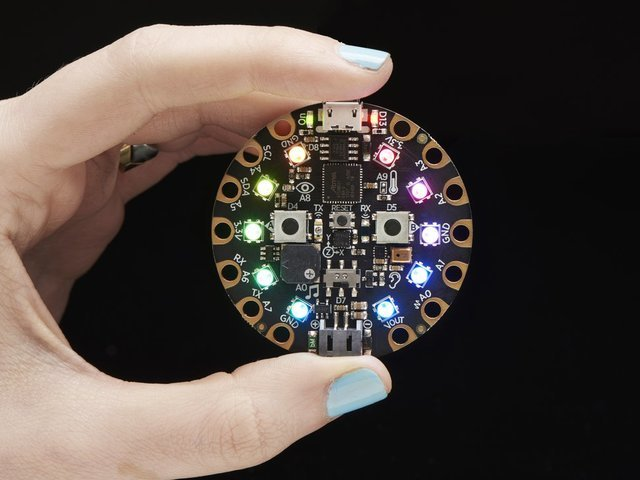
\includegraphics{images/circuit_playground_cpx02.jpg}
\caption{Circuit Playground Express}
\end{figure}

    \textbf{Note:} The Engineering Department will provide you with a
Circuit Playground Express Microcontroller to use during Lab. If you
would like to purchase your own, you can order one here:
\url{https://www.adafruit.com/product/3333}

    On the image of the Circuit Playground Express Microcontroller, label
the following components. Use the following reference:
\url{https://learn.adafruit.com/adafruit-circuit-playground-express/guided-tour}
as a guide.

\begin{itemize}
\tightlist
\item
  microUSB connector
\item
  NeoPixel LED's
\item
  power LED
\item
  buttons
\item
  light sensor
\item
  temperature sensor
\item
  motion sensor
\item
  slide switch
\item
  microphone
\item
  speaker
\end{itemize}

\begin{figure}
\centering
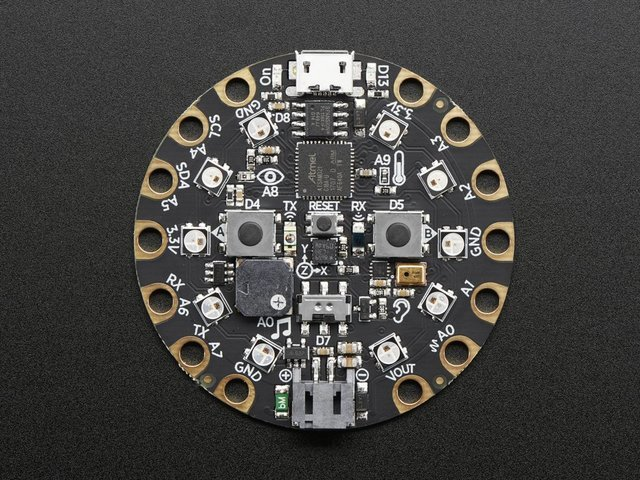
\includegraphics{images/circuit_playground_cpx03.jpg}
\caption{circuit\_playground\_express unlabeled}
\end{figure}

    \hypertarget{connect-the-circuit-playground-express-to-the-computer-and-find-the-file-code.py}{%
\subsubsection{Connect the Circuit Playground Express to the computer
and find the file
code.py}\label{connect-the-circuit-playground-express-to-the-computer-and-find-the-file-code.py}}

Connect the Circuit Playground Express to your computer using a black
microUSB cable. After the Circuit Playground Express is connected, you
should see a new USB device in the Windows file browser.

Open the USB device (like opening a thumb drive) and see the contents.
Note that the file \textbf{\emph{code.py}} is present. We will control
the Circuit Playground Express by modifying the \textbf{\emph{code.py}}
file.

Open Visual Studio Code using the Windows Start Menu. In Visual Studio
Code, select File --\textgreater{} Open Folder and open the USB device.

You should see the file \textbf{\emph{code.py}} in the left-hand file
browser of Visual Studio Code. Double click \textbf{\emph{code.py}} to
open it.

After the Circuit Playground Express is connected to the computer and
\textbf{\emph{code.py}} is open in Visual Studio Code, you are ready to
proceed with the next part of the lab.

    \hypertarget{blink-the-red-led}{%
\subsubsection{Blink the red LED}\label{blink-the-red-led}}

Now we will turn on the red LED on the Circuit Playground Express using
Python.

\begin{figure}
\centering
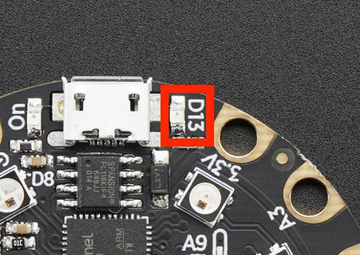
\includegraphics{images/circuitpython_cpx_red_led.jpg}
\caption{Circuit Playground Express Red LED}
\end{figure}

\hypertarget{turn-the-red-led-on}{%
\paragraph{Turn the red LED on}\label{turn-the-red-led-on}}

Open the file \textbf{\emph{code.py}} in a code editor such as VS Code
or Notepad. Copy the code below into \textbf{\emph{code.py}}.

\begin{verbatim}
from adafruit_circuitplayground.express import cpx
     
while True:
    cpx.red_led = True
\end{verbatim}

Save the \textbf{\emph{code.py}} file. Watch the red LED turn on.

\hypertarget{blink-the-red-led-1}{%
\paragraph{Blink the red LED}\label{blink-the-red-led-1}}

If the red LED turns on, the next task is to blink the red LED. Modify
the code in \textbf{\emph{code.py}} with the code below:

\begin{verbatim}
import time
from adafruit_circuitplayground.express import cpx
     
while True:
    cpx.red_led = True
    time.sleep(0.5)
    cpx.red_led = False
    time.sleep(0.5)
\end{verbatim}

Save the \textbf{\emph{code.py}} file. Watch the red LED blink on and
off. Now modify the number in the line \texttt{time.sleep(0.5)} to
something else such as \texttt{time.sleep(2)} or
\texttt{time.sleep(0.2)}. Save \textbf{\emph{code.py}} and observe the
results.

\hypertarget{turn-the-led-on-and-off-with-the-slide-switch}{%
\paragraph{Turn the LED on and off with the slide
switch}\label{turn-the-led-on-and-off-with-the-slide-switch}}

If the red LED blinks on and off, the next task is to turn the red LED
on and off using the slide switch.

\begin{figure}
\centering
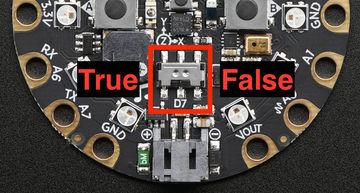
\includegraphics{images/circuitpython_cpx_slide_switch.jpg}
\caption{Circuit Playground Express Slide Switch}
\end{figure}

Modify the code in \textbf{\emph{code.py}} with the code below:

\begin{verbatim}
from adafruit_circuitplayground.express import cpx

while True:
    if cpx.switch:
        cpx.red_led = True
    else:
        cpx.red_led = False
\end{verbatim}

Save \textbf{\emph{code.py}} and slide the switch back and forth. Watch
the LED turn on and off as you slide the switch back and forth.

Now modify the line \texttt{cpx.red\_led\ =\ True} and
\texttt{cpx.red\_led\ =\ False}, to read \texttt{cpx.red\_led\ =\ False}
and \texttt{cpx.red\_led\ =\ True} (switch the \texttt{True} and
\texttt{False} in the code above). Save \textbf{\emph{code.py}}, slide
the switch back and forth and observe the behavior.

    \hypertarget{turn-the-neopixels-on}{%
\subsubsection{Turn the NeoPixels on}\label{turn-the-neopixels-on}}

If the slide switch turns the red LED on and off, the next task is to
turn the Circuit Playground Express NeoPixels on and off. The NeoPixels
are the 10 ``white'' LED's that form a circle around the Circuit
Playground Express.

\begin{figure}
\centering
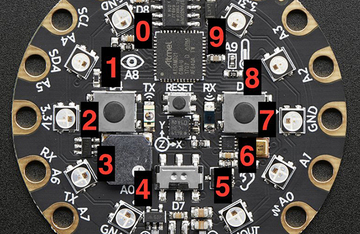
\includegraphics{images/circuitpython_cpx_neopixel_numbering.jpg}
\caption{NeoPixel Numbering}
\end{figure}

\hypertarget{turn-a-neopixels-red}{%
\paragraph{Turn a NeoPixels red}\label{turn-a-neopixels-red}}

First, we will make one of the NeoPixels red. Modify the code in
\textbf{\emph{code.py}} with the code below:

\begin{verbatim}
from adafruit_circuitplayground.express import cpx

cpx.pixels.brightness = 0.3

while True:
    cpx.pixels[0] = (255, 0, 0)
\end{verbatim}

Save \textbf{\emph{code.py}} and watch one of the NeoPixels turn red.

Now modify the line \texttt{cpx.pixels{[}0{]}\ =\ (255,\ 0,\ 0)} to turn
on one of the other NeoPixels on. Try
\texttt{cpx.pixels{[}1{]}\ =\ (255,\ 0,\ 0)}. Remember to save your
\textbf{\emph{code.py}} file after you make changes.

\hypertarget{turn-a-neopixel-green-then-other-colors}{%
\paragraph{Turn a NeoPixel green then other
colors}\label{turn-a-neopixel-green-then-other-colors}}

After you are able to turn different NeoPixels red, the next thing we
will do is change the color of the NeoPixels. Modify the code in
\textbf{\emph{code.py}} with the code below. Note the only difference
from the code above are the numbers in parentheses
\texttt{(0,\ 255,\ 0)} on the last line.

\begin{verbatim}
from adafruit_circuitplayground.express import cpx

cpx.pixels.brightness = 0.3

while True:
    cpx.pixels[0] = (0, 255, 0)
\end{verbatim}

Save \textbf{\emph{code.py}} and watch one of the NeoPixels turn green.
Now try a couple other colors. For example, the line
\texttt{cpx.pixels{[}0{]}\ =\ (0,\ 0,\ 255)} will turn the NeoPixel
blue.

\hypertarget{turn-on-multiple-neopixels-at-the-same-time}{%
\paragraph{Turn on multiple NeoPixels at the same
time}\label{turn-on-multiple-neopixels-at-the-same-time}}

Now that you can change the color of a NeoPixel, the next task is to
turn on two NeoPixels at the same time. Modify the code in
\textbf{\emph{code.py}} with the code below:

\begin{verbatim}
from adafruit_circuitplayground.express import cpx

cpx.pixels.brightness = 0.3

while True:
    cpx.pixels[0] = (255, 0, 0)
    cpx.pixels[1] = (0, 255, 0)
    cpx.pixels[2] = (0, 0, 255)
\end{verbatim}

Save \textbf{\emph{code.py}} and watch two NeoPixels light up at the
same time. Now modify the code in \textbf{\emph{code.py}} to turn on
even more of the NeoPixels. Note you will have to add another line such
as \texttt{cpx.pixels{[}3{]}\ =\ (0,\ 0,\ 255)} to the end of the
\textbf{\emph{code.py}} file to accomplish this. Continue to modify
\textbf{\emph{code.py}} until you turn all 10 of the NeoPixels on at the
same time.

\hypertarget{build-a-neopixel-rainbow}{%
\paragraph{Build a NeoPixel Rainbow}\label{build-a-neopixel-rainbow}}

After you turn on all of the NeoPixels on, modify the code in
\textbf{\emph{code.py}} to create a NeoPixel rainbow. Use the code below
as a starting point. Look up RGB color values on the internet. For
example, yellow is \texttt{(225,\ 255,\ 0)}.

\begin{verbatim}
from adafruit_circuitplayground.express import cpx

cpx.pixels.brightness = 0.3

while True:
    cpx.pixels[0] = (255, 0, 0)
    cpx.pixels[1] = (225, 255, 0)
    cpx.pixels[2] = (255, 165, 0) 
\end{verbatim}

    \hypertarget{use-the-light-sensor}{%
\subsubsection{Use the light sensor}\label{use-the-light-sensor}}

After you are able to blink the red LED on and off and build a NeoPixel
rainbow, the next thing we will do is use the Circuit Playground Express
light sensor.

\begin{figure}
\centering
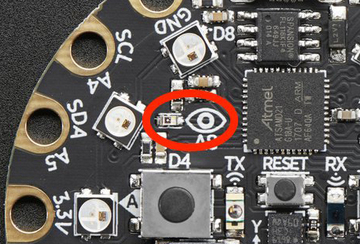
\includegraphics{images/circuitpython_cpx_light_sensor.jpg}
\caption{Circuit Playground Express Light Sensor}
\end{figure}

\hypertarget{use-the-slide-switch-to-turn-on-the-neopixels}{%
\paragraph{Use the slide switch to turn on the
NeoPixels}\label{use-the-slide-switch-to-turn-on-the-neopixels}}

Before we use the light sensor, let's use the slide switch to turn the
NeoPixel LED's on and off. Modify the code in \textbf{\emph{code.py}}
with the code below and save it. Indentation is important in Python.
Make sure your indentation is exactly like the code listed.

\begin{verbatim}
from adafruit_circuitplayground.express import cpx

cpx.pixels.brightness = 0.3

while True:
    if cpx.switch:
        cpx.pixels[0] = (255, 0, 0)
    else:
        cpx.pixels[0] = (0, 0, 0)
\end{verbatim}

Slide the switch back and forth and watch the NeoPixel turn on. Now
modify the code so that all the NeoPixels turn on with the slide switch.
The code below gives you a hint on how to do this. Remember to save
\textbf{\emph{code.py}} after you make changes.

\begin{verbatim}
from adafruit_circuitplayground.express import cpx

cpx.pixels.brightness = 0.3

while True:
    if cpx.switch:
        cpx.pixels[0] = (255, 0, 0)
        cpx.pixels[1] = (255, 255, 0)
        cpx.pixels[2] = (255, 165, 0)
        ...
    else:
        cpx.pixels[0] = (0, 0, 0)
        cpx.pixels[1] = (0, 0, 0)
        cpx.pixels[2] = (0, 0, 0)
        ...
\end{verbatim}

Now modify the code so that the slide switch produces different patterns
of NeoPixel light. You could try to make all the NeoPixels red when the
switch is on one side and then all the NeoPixels green when the switch
is on the other side.

\hypertarget{use-the-light-sensor-to-turn-on-the-neopixels}{%
\paragraph{Use the light sensor to turn on the
NeoPixels}\label{use-the-light-sensor-to-turn-on-the-neopixels}}

After you can change the NeoPixels with the slide switch, the next task
is to use the light sensor on the Circuit Playground express. The code
below will turn on the NeoPixels based on the brightness recorded by the
light sensor. Make sure to copy the code exactly and pay attention to
indentation. Remember that indentation is important in Python.

\begin{verbatim}
import time
from adafruit_circuitplayground.express import cpx
import simpleio

cpx.pixels.auto_write = False
cpx.pixels.brightness = 0.3

while True:
    # light value remapped to pixel position
    peak = simpleio.map_range(cpx.light, 0, 320, 0, 10)
    for i in range(0, 10, 1):
        if i <= peak:
            cpx.pixels[i] = (0, 255, 255)
        else:
            cpx.pixels[i] = (0, 0, 0)
    cpx.pixels.show()
    time.sleep(0.05)
\end{verbatim}

Put your finger over the light sensor and see the results. See if you
can make the color of the NeoPixels change based on light sensor input
by modifying the line \texttt{cpx.pixels{[}i{]}\ =\ (0,\ 255,\ 255)}.
You may need to add a few lines as well. Don't be afraid of breaking the
Circuit Playground Express. Just try to modify the code in
\textbf{\emph{code.py}} and see the results.

    \hypertarget{use-the-accelerometer}{%
\subsubsection{Use the accelerometer}\label{use-the-accelerometer}}

After you succeed in getting the light sensor to turn the NeoPixels on
and off, the next part of the Circuit Playground express we will use is
the accelerometer. An accelerometer measures acceleration. If three
accelerometers are mounted in a device in different orientations,
accelerometers can also be used to calculate the tilt of a device, or
how the device is rotated.

\begin{figure}
\centering
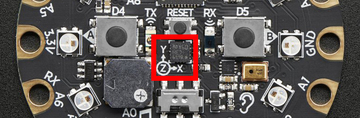
\includegraphics{images/circuitpython_cpx_accelerometer.jpg}
\caption{Circuit Playground Express Accelerometer}
\end{figure}

Modify the code in \textbf{\emph{code.py}} with the code below and save
it.

\begin{verbatim}
from adafruit_circuitplayground.express import cpx

# Main loop gets x, y and z axis acceleration, prints the values, and turns on
# red, green and blue, at levels related to the x, y and z values.
while True:
    if cpx.switch:
        print("Slide switch off!")
        cpx.pixels.fill((0, 0, 0))
        continue
    else:
        R = 0
        G = 0
        B = 0
        x, y, z = cpx.acceleration
        print((x, y, z))
        if x:
            R = R + abs(int(x))
        if y:
            G = G + abs(int(y))
        if z:
            B = B + abs(int(z))
        cpx.pixels.fill((R, G, B))
\end{verbatim}

After \textbf{\emph{code.py}} is saved, pick up the Circuit Playground
Express and move it around. See how the NeoPixels change color when the
device is rotated.

    \hypertarget{try-something-on-your-own}{%
\subsubsection{Try something on your
own}\label{try-something-on-your-own}}

After you succeed in getting the accelerometer to turn the NeoPixels
different colors, it is time for you to try something on your own.
Browse to the following page
\url{https://learn.adafruit.com/circuitpython-made-easy-on-circuit-playground-express/acceleration}
and view the options down the left hand side. Some of the options are:

\begin{itemize}
\tightlist
\item
  Buttons
\item
  Temperature
\item
  Capacitive Touch
\item
  Play Tone
\end{itemize}

Pick one of these options. Copy the code from the webpage into
\textbf{\emph{code.py}} and see the results. In the space below, write a
couple sentences that describes what you did. You can also try something
totally different that's not listed on the web page.

\begin{verbatim}











\end{verbatim}
\newpage
    \hypertarget{self-reflection}{%
\subsubsection{Self Reflection}\label{self-reflection}}

Before you leave lab, complete the following self-reflection questions.
Record your answers below.

\begin{enumerate}
\def\labelenumi{\arabic{enumi}.}
\tightlist
\item
  How confident were you going into lab today knowing that you would
  have to write some programming code? What were you most worried about,
  what were you most prepared for?
\end{enumerate}

\begin{verbatim}

















\end{verbatim}

\begin{enumerate}
\def\labelenumi{\arabic{enumi}.}
\setcounter{enumi}{1}
\tightlist
\item
  What did you find easy in the lab today? Which tasks did you complete
  quickly without any help?
\end{enumerate}

\begin{verbatim}
























\end{verbatim}

\begin{enumerate}
\def\labelenumi{\arabic{enumi}.}
\setcounter{enumi}{2}
\tightlist
\item
  What stumbling blocks or challenges did you encounter during lab? What
  did you find hard and took the most time?
\end{enumerate}

\begin{verbatim}


















\end{verbatim}

\begin{enumerate}
\def\labelenumi{\arabic{enumi}.}
\setcounter{enumi}{3}
\tightlist
\item
  How did you address these stumbling blocks or challenges? (Asked a
  partner, asked the instructor, looked for help online, etc).
\end{enumerate}

\begin{verbatim}


























\end{verbatim}

\begin{enumerate}
\def\labelenumi{\arabic{enumi}.}
\setcounter{enumi}{4}
\tightlist
\item
  What advice would you give to future students before they start the
  lab? What did you wish you'd known before you started the lab?
\end{enumerate}

\begin{verbatim}
































\end{verbatim}

    \hypertarget{tipsreminders}{%
\subsubsection{Tips/reminders}\label{tipsreminders}}

\begin{itemize}
\item
  It is really hard to break a Circuit Playground Express. As long as
  you don't throw the device across the room, or hit it with a hammer,
  the very worst thing that can happen is that you have to unplug the
  Circuit Playground Express and restart your computer. Play around with
  the code and try new things. You won't break anything.
\item
  Remember that Python is case sensitive. Capital \texttt{A} and
  lowercase \texttt{a} are different in Python. Pay attention to the
  words \texttt{True} and \texttt{true}. Python treats these two
  keywords differently.
\item
  Remember that indentation is import in Python. If the indentation of
  Python code is not entered correctly, the code will not run as
  expected.
\item
  Remember to use colons (\texttt{:}) where noted. It is easy to forget
  colons at the end of certain code lines.
\item
  Generally, spaces in lines of Python code don't make a difference. But
  be careful with parenthesis \texttt{(\ )} and square brackets
  \texttt{{[}\ {]}}.
\end{itemize}

    \hypertarget{deliverable}{%
\subsection{Deliverable}\label{deliverable}}

Hand in a hard copy of your lab by the end of the lab period to your
instructor. Make sure you have filled out the \textbf{Try something on
your own} section and the \textbf{self-reflection questions}. Make sure
your lab has your name on it. \textbf{Students who do not put their name
on their papers will not receive credit for the lab.}

    \hypertarget{by-p.-kazarinoff-portland-community-college-2019}{%
\paragraph{\texorpdfstring{\emph{By P. Kazarinoff, Portland Community
College,
2019}}{By P. Kazarinoff, Portland Community College, 2019}}\label{by-p.-kazarinoff-portland-community-college-2019}}


    % Add a bibliography block to the postdoc
    
    
    
    \end{document}
